% ═════════════════════════════════════════════════════════════════════════════
%  The Shape of Evidence: Fuzzy Prediction Sets for Downstream Decisions
%  MSc Quantitative Finance, Erasmus School of Economics
%
%  Build:  pdflatex main  ->  bibtex main  ->  pdflatex main  ->  pdflatex main
%  Figures in ../code/figures/ are produced by decision_pipeline.py
% ═════════════════════════════════════════════════════════════════════════════
\documentclass[11pt, a4paper]{article}

% ═════════════════════════════════════════════════════════════════════════════
%  PREAMBLE
% ═════════════════════════════════════════════════════════════════════════════

% ── Encoding and fonts ───────────────────────────────────────────────────────
\usepackage[T1]{fontenc}
\usepackage[utf8]{inputenc}
\usepackage{lmodern}
\usepackage[english]{babel}

% ── Page geometry ────────────────────────────────────────────────────────────
% Conventional thesis page: 11pt body, margins near 3 cm with a little extra
% on the binding edge, giving a measure of roughly 85 characters.
\usepackage[a4paper, inner=2.9cm, outer=2.7cm, top=2.5cm, bottom=2.7cm,
            headheight=14pt, headsep=13pt]{geometry}
\usepackage{setspace}
% 1.3 keeps the lines clearly separated at this measure while fitting
% appreciably more text per page than one-and-a-half spacing.
\setstretch{1.23}

% ── Mathematics ──────────────────────────────────────────────────────────────
\usepackage{amsmath, amssymb, amsthm}
% Number equations by section (2.1, 2.2, ...) rather than continuously, so a
% reference locates the equation as well as naming it.
\numberwithin{equation}{section}

% ── Tables and figures ───────────────────────────────────────────────────────
\usepackage{graphicx}
% Figures have one source of truth: analysis/results/figures/. The relative path keeps the
% paper reproducible without maintaining a second, potentially stale, copy.
\graphicspath{{../analysis/results/figures/}{assets/}{./}}
\usepackage{booktabs}
\usepackage{array}
% Booktabs rules need room to breathe; the default row height crowds them.
\renewcommand{\arraystretch}{1.18}
\usepackage{float}
\usepackage[font=small, labelfont=bf, labelsep=period,
            width=0.94\textwidth, justification=justified,
            singlelinecheck=true]{caption}

% ── Lists, headers, references ───────────────────────────────────────────────
\usepackage{enumitem}
\setlist[enumerate]{itemsep=2pt, topsep=4pt}
\setlist[itemize]{itemsep=2pt, topsep=4pt}
\usepackage{natbib}
\bibliographystyle{plainnat}
\usepackage{fancyhdr}
\usepackage{titlesec}
\usepackage{tocloft}
% Open up the contents list: entries are few, so they can afford the space.
\setlength{\cftbeforesecskip}{0.7em}
\setlength{\cftbeforesubsecskip}{0.25em}
\renewcommand{\cftsecfont}{\bfseries}
\renewcommand{\cftsecpagefont}{\bfseries}
\renewcommand{\cftsecleader}{\cftdotfill{\cftdotsep}}
\renewcommand{\cftsubsecleader}{\hfill}
\renewcommand{\cftsubsecafterpnum}{\hspace*{0pt}}
\usepackage{microtype}

% ── Hyperlinks (loaded late) ─────────────────────────────────────────────────
\usepackage{xcolor}
\definecolor{linknavy}{RGB}{20,60,110}
\definecolor{citeink}{RGB}{55,70,95}
\usepackage[hidelinks]{hyperref}
% Long dataset URLs cannot be hyphenated; let them break at any character so a
% single reference does not force loose lines through the whole entry.
\usepackage{url}
\def\UrlBreaks{\do\/\do-\do.\do:\do_\do?\do\&\do=\do+}
\Urlmuskip=0mu plus 2mu
\hypersetup{
  colorlinks = true,
  linkcolor  = citeink,
  citecolor  = citeink,
  urlcolor   = linknavy,
  pdftitle   = {The Shape of Evidence: Fuzzy Prediction Sets for Downstream Decisions},
  pdfauthor  = {Antonis Konstantinidis},
  bookmarksnumbered = true
}

% ═════════════════════════════════════════════════════════════════════════════
%  STYLING
% ═════════════════════════════════════════════════════════════════════════════

% Running header: section name left, page number right, set in small caps so
% it recedes behind the text rather than competing with the headings.
\pagestyle{fancy}
\fancyhf{}
\renewcommand{\headrulewidth}{0.4pt}
\fancyhead[L]{\footnotesize\scshape\nouppercase{\leftmark}}
\fancyhead[R]{\footnotesize\thepage}
\fancypagestyle{plain}{\fancyhf{}\renewcommand{\headrulewidth}{0pt}%
  \fancyfoot[C]{\footnotesize\thepage}}

% Section headings. Generous space above, tighter below, so each heading binds
% to the text it introduces rather than floating between blocks.
\titleformat{\section}{\normalfont\Large\bfseries}{\thesection}{0.7em}{}
\titleformat{\subsection}{\normalfont\large\bfseries}{\thesubsection}{0.7em}{}
% Every major section starts on a new page. Subsections remain attached to the
% surrounding text because they mark divisions within a section, not new
% chapters.
\titlespacing*{\section}{0pt}{3.4ex plus 1ex minus .3ex}{1.5ex plus .2ex}
\titlespacing*{\subsection}{0pt}{2.4ex plus .8ex minus .2ex}{0.9ex plus .2ex}
\newcommand{\sectionbreak}{\clearpage}

% Floats: keep them clear of the surrounding text.
\setlength{\textfloatsep}{14pt plus 3pt minus 3pt}
\setlength{\intextsep}{12pt plus 3pt minus 3pt}
\setlength{\abovecaptionskip}{7pt}
\setlength{\belowcaptionskip}{2pt}

% Display equations and the operators inside them get more air. Size commands
% reset the display skips, so they are reapplied whenever \normalsize runs.
\newcommand{\displayair}{%
  \setlength{\abovedisplayskip}{13pt plus 3pt minus 2pt}%
  \setlength{\belowdisplayskip}{13pt plus 3pt minus 2pt}%
  \setlength{\abovedisplayshortskip}{8pt plus 3pt}%
  \setlength{\belowdisplayshortskip}{10pt plus 3pt}}
\usepackage{etoolbox}
\appto{\normalsize}{\displayair}
\AtBeginDocument{\displayair}
\setlength{\jot}{6pt}
\medmuskip=4.5mu plus 2mu minus 2mu
\thickmuskip=6mu plus 4mu minus 1mu

% Discourage widows and orphans.
\widowpenalty=10000
\clubpenalty=10000

% ═════════════════════════════════════════════════════════════════════════════
%  THEOREM ENVIRONMENTS
% ═════════════════════════════════════════════════════════════════════════════
% Theorem-like results are separated from the prose that frames them.
\newlength{\thmsep}\setlength{\thmsep}{1.1\baselineskip}
\makeatletter
\def\thm@space@setup{%
  \thm@preskip=\thmsep \thm@postskip=\thmsep}
\makeatother
\theoremstyle{plain}
\newtheorem{theorem}{Theorem}[section]
\newtheorem{proposition}[theorem]{Proposition}
\newtheorem{lemma}[theorem]{Lemma}
\newtheorem{corollary}[theorem]{Corollary}
\theoremstyle{definition}
\newtheorem{definition}[theorem]{Definition}
\theoremstyle{remark}
\newtheorem{remark}[theorem]{Remark}

% ═════════════════════════════════════════════════════════════════════════════
%  MATH SHORTHAND
% ═════════════════════════════════════════════════════════════════════════════
\DeclareMathOperator*{\argmin}{arg\,min}



\begin{document}

% ── TITLE PAGE ───────────────────────────────────────────────────────────────
\begin{titlepage}
\centering
\thispagestyle{empty}
\hypersetup{pageanchor=false}
% The body measure is wide for density; a title page set to that full width
% looks stretched, so the whole block is inset and centred on the page.
\newlength{\titlemeasure}\setlength{\titlemeasure}{0.78\textwidth}
\begin{minipage}[c][0.96\textheight][s]{\titlemeasure}
\centering


\includegraphics[width=5.2cm]{assets/eur.png}\\[1.6em]
{\scshape\large Erasmus School of Economics}\\[0.35em]
{\scshape MSc Quantitative Finance}\\[0.35em]
{\small Academic Year 2025--2026}

\vfill

\rule{\titlemeasure}{1.2pt}\\[1.1em]
{\Huge\bfseries The Shape of Evidence}\\[0.9em]
{\LARGE Fuzzy Prediction Sets for Downstream Decisions}\\[1.1em]
\rule{\titlemeasure}{1.2pt}

\vspace{2.2em}

{\large\bfseries Antonis Konstantinidis}\\[0.4em]
{\small Student ID: 656699}

\vfill

\begin{tabular}{@{}r@{\hskip 1.2em}l@{}}
\textit{Supervisor} & Dr.\ Nick Koning \\[0.3em]
\textit{Date}       & \monthyear
\end{tabular}\par
\end{minipage}

\end{titlepage}

% ── FRONT MATTER ─────────────────────────────────────────────────────────────
\pagenumbering{roman}
\setcounter{page}{2}
\hypersetup{pageanchor=true}

% Abstract set on its own page, inset from the body measure so it reads as a
% standalone summary rather than a stray first page.
\thispagestyle{empty}
\begin{center}
\begin{minipage}{0.80\textwidth}
\setlength{\parindent}{1.5em}
\begin{center}\large\bfseries Abstract\end{center}
\vspace{0.6em}
\begin{spacing}{1.15}
\noindentSound statistical evidence does not guarantee good decisions. Consider a
decision-maker whose loss depends on which outcome occurs. They ask a
statistician for a report that scores each outcome by how strongly the data
count against it, and the report must be valid, misleading no more often than
a pre-agreed rate. Many reports may be valid, yet recommend different actions.
Existing theory picks the report that accumulates evidence fastest, without
considering the decision-maker's losses at stake. This thesis instead asks which report to
choose when such loss function is known in advance.

Each report bounds an action's expected loss. The ``safe'' report minimises
this bound by scoring outcomes in proportion to the action's losses, and
leads to the action it ``protects''. By contrast, the report that
accumulates evidence fastest may recommend a different action, in which case
the protected action must be imposed as a constraint. That report scores
outcomes by how much likelier the data make them, and recovers the safe report
only when losses follow those likelihoods.

For a shopkeeper ordering shirts before the 2026 World Cup final, with
Polymarket prices as the forecast, no likelihood-based report found in two
searches selects the order the forecast recommends, unlike the safe report. In
controlled simulations, the likelihood-based report picks the wrong action
even when the forecast is right. Losses belong in the design of evidence, not
its interpretation.

\end{spacing}

\vspace{2.2em}
\begin{center}\bfseries Acknowledgements\end{center}
\vspace{0.4em}
\begin{spacing}{1.15}
\noindent I would like to thank my supervisor, Dr.\ Nick Koning, for his guidance
and constructive feedback throughout this thesis. His support was instrumental
in shaping the direction and clarity of my work. I also extend my appreciation
to the staff and students of the Erasmus School of Economics for providing a
stimulating and supportive academic environment.
\end{spacing}
\end{minipage}
\end{center}
\vfill

\newpage
\begin{spacing}{1.06}
\tableofcontents
\end{spacing}

% ── BODY ─────────────────────────────────────────────────────────────────────
\pagenumbering{arabic}

%═══════════════════════════════════════════════════════════════════════════════
\section{Introduction}\label{sec:introduction}
%═══════════════════════════════════════════════════════════════════════════════

\subsection{From Prediction Sets to Scores}\label{sec:intro_sets}

Consider a decision-maker who must act before an uncertain outcome is known.
They know which outcomes may occur, which actions are available to take, and what each
action would cost in each outcome. What they do not know is which outcome will
occur, so they ask a statistician for evidence.

Call whatever the statistician sends back a report. It might be a shortlist of
the outcomes still worth taking seriously, or a score for each outcome saying
how strongly the data count against it. Whatever its form, a report must be
valid, meaning it must not mislead more often than a pre-agreed error rate allows.

The established way to build such a report is to build a
prediction set, a shortlist of the outcomes that remain plausible. Conformal
prediction constructs such sets with a coverage guarantee: for a chosen level
$\alpha\in(0,1)$, the shortlist $S$ contains the realised outcome $Z$ with
probability at least $1-\alpha$, that is, $P[Z\in S]\geq1-\alpha$
\citep{vovk2005,angelopoulos2023conformal}. A cautious decision-maker can then
protect against the worst thing the shortlist still permits,
\begin{equation}
  \delta_S\in\argmin_{d\in\mathcal D}\ \max_{z\in S}L(d,z),
  \label{eq:intro_set_rule}
\end{equation}
writing $L(d,z)$ for what action $d$ costs when outcome $z$ occurs. Whenever
the realised outcome lies in $S$, the loss of $\delta_S$ cannot exceed the
worst loss over $S$, so coverage carries over to the decision,
\begin{equation}
  P\Big[L(\delta_S,Z)\leq\max_{z\in S}L(\delta_S,z)\Big]\geq1-\alpha .
  \label{eq:intro_set_guarantee}
\end{equation}
This is the basis of certified-decision methods
\citep{AndrewsChen2025,Kiyani2025}.

This guarantee is genuine, but a shortlist records only membership. Once two
outcomes are both in it, the set no longer says which one the data support
more strongly, so the rule treats a barely plausible outcome and a highly
likely one identically. The recommended action can also change with the
coverage level even though nothing about the decision has changed.

E-values keep what a shortlist discards. Rather than sorting each outcome in
or out, they give every outcome its own score $\mathcal E(z)\geq0$, large
where the data argue against that outcome and small where they do not. The
collection of these scores, one per outcome, is what the statistician hands
over. This thesis calls it a profile and writes it $\mathcal E$.

What stops a profile from claiming strong evidence everywhere is a single
requirement,
\begin{equation}
  \mathbb E_{P}[\mathcal E(Z)]\leq 1 ,
  \label{eq:intro_validity}
\end{equation}
that the scores average to at most one under the distribution $P$ the evidence
is weighed against. Section~\ref{sec:decision} extends this to a whole set
$\mathcal P$ of distributions.

A profile satisfying this restriction is valid, and a valid profile is also
called an e-variable. The condition acts as a budget: raising the score on one outcome forces a reduction elsewhere. In return, the scores can be compared against any threshold, even one chosen after they are seen, without losing the guarantee (Section~\ref{sec:evar}). This is the basis of safe
testing \citep{Shafer2021,Grunwald2024safe,Ramdas2023}. Fuzzy prediction sets
carry this graded evidence back to the prediction problem, replacing the
in-or-out verdict of a shortlist with a score for every outcome
\citep{KoningvanMeer2025,Vovk2025,Gauthier2025}.

\subsection{Two Ways to Judge a Profile}\label{sec:intro_two}

Validity rules out overclaiming, but it leaves a great deal open. Many
profiles satisfy it, and they need not lead the decision-maker to the same
action. The statistician must still choose one, and could let what each
mistake would cost guide that choice. This is where the existing literature
and the decision-maker part company.

The standard construction compares two distributions. One is $P$, the
distribution validity is required to hold under. The other is the belief $\widehat P_1$,
what the decision-maker expects to happen. Their ratio
\begin{equation}
  r(z):=\frac{\widehat P_1(z)}{P(z)}
  \label{eq:intro_lr}
\end{equation}
is large where the belief rates an outcome likelier than $P$ does, and the profile is built by passing this ratio through an increasing
shape function $w$, reporting $\mathcal E(z)=w(r(z))$. 

The usual measure of how much a profile tells us is its expected
log-evidence under the belief, $\mathbb E_{\widehat P_1}[\log\mathcal E(Z)]$,
which is high when large scores sit where the belief puts its probability.
Whenever $P$ gives every outcome positive probability, $w(r)=r$ maximises it
among valid profiles \citep{Grunwald2024safe,Koning2025continuous}. Statisticians with other preferences over how evidence accumulates choose
other shape functions, and \citet{KoningvanMeer2025} determine which $w$ is
best once such a preference is fixed.

However, all of this concerns how much the evidence tells us. It says nothing about
what happens when the evidence must produce an action. For that,
\citet{KoningvanMeer2025} score each action by
\begin{equation}
  C(d;\mathcal E):=\max_{z\in\mathcal Z}\frac{L(d,z)}{\mathcal E(z)} ,
  \label{eq:intro_cert}
\end{equation}
its largest loss across outcomes, with each loss first divided by the evidence
against the outcome that would produce it. Validity turns this single number
into a bound on the action's expected loss, and the decision-maker takes
whichever action has the smallest one.

Dividing by the score is how evidence lowers the bound. A large score on an
outcome shrinks the loss the action would suffer there, while a small score
leaves that loss large. Because of the budget, the scores cannot all be large,
so a profile has to choose where its large scores go.
The bound is the worst loss after division, so it stays low only if the large
scores sit where the action's losses are large.

This is where the standard construction can go wrong. It puts its large
scores on the outcomes the belief expects, those that $\widehat P_1$ rates
likelier than $P$ does, and is therefore left with small scores on the
outcomes the belief considers unlikely. If the action is expensive in
one of those unlikely outcomes, that loss is not reduced, and the action's
bound is poor. Which outcomes the belief expects and where the
decision-maker has most to lose are separate questions, and there is no
reason their answers should coincide.

An evidence profile can thus be judged in two ways, by the information it preserves, or
by the protection it gives to a decision. The two judgements need not agree, which leads to
the research question of the thesis:
\begin{quote}
Given a loss function and a stated attitude toward risk, how should a
statistician choose the e-variable supplied to a decision-maker?
\end{quote}

\subsection{Contribution}\label{sec:intro_contrib}

Existing theory chooses a profile by a preference over evidence, and cannot
say which preference represents a given decision-maker's loss. The closest predecessor is
the e-posterior of \citet{Grunwald2023epost}, which supports frequentist
decision-making without a prior and already divides a loss by an e-value in
the manner of \eqref{eq:intro_cert}. Neither supplies a design step in which the loss
function is an input to the construction of the profile itself. This step is the contribution of
this thesis, which uses three results to answer the question.

The first asks how low the bound on a chosen action's loss can be pushed. The
answer is to make the scores proportional to what that action costs in each
outcome, and the bound then equals that action's largest expected loss across
the distributions validity must hold under (Theorem~\ref{thm:cert}). No other
valid profile does as well, and the optimum is unique. Call it the safe
profile. It is built from the loss and those distributions alone, while the
belief plays no part in it.

The second result separates informing from inducing. The safe profile
always leads to the action it protects, unless some other action is cheaper in
every outcome, but the most informative profile, the likelihood ratio, need
not, even when the target is the action the belief
itself favours. Keeping as much information as possible while still reaching
the target therefore requires imposing the target as a constraint, and the
optimum then sits where the target ties with a competitor
(Proposition~\ref{prop:boundary}).

The third asks whether the standard construction could have found the
safe profile anyway. Since it reads each outcome only through $r$, two
outcomes with the same likelihood ratio must receive the same score, however
differently they cost. The safe profile is built from the loss
and can separate them. The two agree exactly when the loss is determined by
the ratio (Proposition~\ref{prop:no_shape}). Otherwise, no shape function
recovers the safe profile, so the loss must enter the design of the
profile rather than be applied to its output.
%═══════════════════════════════════════════════════════════════════════════════
\section{Theoretical Framework}\label{sec:decision}
%═══════════════════════════════════════════════════════════════════════════════

\subsection{The Decision Problem}\label{sec:problem}

Let $Z$ be an unknown outcome in a finite outcome space $\mathcal Z$, and let
$d\in\mathcal D$ be an action chosen before $Z$ is observed. The loss
$L(d,z)\geq0$ is what choosing $d$ costs when the outcome turns out to be $z$.
The decision-maker supplies this loss table, and it records which mistakes
matter and by how much. With finitely many outcomes the table is a grid of
numbers, one per action and outcome, and $L(d,\cdot)$ denotes the row for
action $d$, listing what that action costs in each outcome in turn.

Uncertainty about outcome $Z$ enters in two separate places. The first is the model $\mathcal P$, a set of distributions any one of which
could be the true one. The decision-maker is unwilling to stake the guarantee
on a single distribution, so the report is required to be valid under every
member at once. As $\mathcal P$ gets larger, the statement about what
the world might be doing becomes more cautious, and it buys a weaker guarantee in return.

The second is the belief $\widehat P_1$, the single distribution the
decision-maker actually thinks is true, formed before any data is collected.
It carries no guarantee whatever. Intuitively, it is simply what they would act on ``if
nothing could go wrong''.

The two do different jobs. The model says what the report must survive, the
belief says what it should be good at. They are not competing estimates of one
quantity, and the thesis is about what happens when they disagree about which
action to take. Two standing assumptions apply throughout: every distribution
in $\mathcal P$ gives every outcome positive probability, so each expected
loss is a finite sum, and every expectation is taken under the distribution
named in its subscript.

\subsection{Evidence Profiles and Validity}\label{sec:evar}

A profile $\mathcal E$ is a valid e-variable for the model $\mathcal P$ when
\begin{equation}
  \mathbb E_{P}[\mathcal E(Z)]\leq1
  \qquad\text{for every }P\in\mathcal P .
  \label{eq:evalue_def}
\end{equation}

Read as a budget, the condition gives the profile one unit of e-value to spend
on average. Nothing dictates how that unit is spread across outcomes, and how to spread it is precisely the design problem of this
thesis. Constructing a valid profile from raw data is a separate problem,
solved by the methods cited in Section~\ref{sec:introduction}, and is taken as
given here.

What makes the condition worth accepting is what it buys. Markov's inequality
turns it into
\begin{equation}
  P[\mathcal E(Z)\geq1/\alpha]\leq\alpha
  \qquad\text{for every }\alpha\in(0,1),
  \label{eq:markov}
\end{equation}
so a profile whose score at an outcome exceeds $1/\alpha$ can be treated as
evidence at level $\alpha$ against it. This holds at every $\alpha$
simultaneously and under every member of the model, so a single profile serves
every threshold a reader might apply with no correction for inspecting
several. A companion result \citep{Grunwald2024,Koning2024posthoc} extends it
to thresholds chosen after the scores are seen, so evidence can be published
before anyone fixes how strictly to read it.

One further consequence matters below. Only the hardest constraint in
\eqref{eq:evalue_def} does any work: the profile is valid exactly when its
largest expectation across the model is at most one, so validity is settled by
the single member under which the profile looks largest. A profile
that spends the budget exactly under some member, rather than leaving slack
everywhere, is the interesting case, since any leftover could be spent on
sharper evidence. Every profile constructed in this thesis is of that kind. The
examples below use the simplest model, a single distribution
$\mathcal P=\{P_0\}$, to keep the arithmetic checkable, and
Section~\ref{sec:market} uses a genuinely composite one.

\subsection{From Prediction Sets to the Weighted Rule}\label{sec:rule}

A profile has to become an action. For a prediction set this is done by the
rule \eqref{eq:intro_set_rule}, which protects against the worst outcome the
set still admits. The profile analogue replaces the worst case over a set by a
worst case weighted by the evidence. This is the weighted worst-case rule of
\citet{KoningvanMeer2025},
\begin{equation}
  \delta(\mathcal E)\in\argmin_{d\in\mathcal D}C(d;\mathcal E),
  \qquad
  C(d;\mathcal E):=\max_{z\in\mathcal Z}
  \frac{L(d,z)}{\mathcal E(z)},
  \label{eq:wl_decision}
\end{equation}
with the conventions $x/0=\infty$ for $x>0$ and $0/0=0$. Dividing by the score
does not declare an outcome impossible: it discounts a loss that would be
incurred only if the outcome occurred, in proportion to the evidence against
it.

The number $C(d;\mathcal E)$ is called the certificate of $d$, because it
bounds expected loss. It depends only on the loss row and the profile, so it
is known before the outcome is. Assume $C(d;\mathcal E)<\infty$, since otherwise the
bound is vacuous. By definition of the maximum,
$L(d,z)\leq C(d;\mathcal E)\,\mathcal E(z)$ at every outcome, so for any
$P\in\mathcal P$,
\begin{equation}
  \mathbb E_{P}[L(d,Z)]
  \leq C(d;\mathcal E)\,\mathbb E_{P}[\mathcal E(Z)]
  \leq C(d;\mathcal E).
  \label{eq:cert_bound}
\end{equation}
The final inequality is where validity is used, and without it a profile could
be scaled up to make any certificate small. The bound holds under every
member of the model at once, and it concerns expected loss, not every realised
loss. The same pointwise inequality also gives a tail bound. A loss of at
least $C(d;\mathcal E)/\alpha$ forces a score of at least $1/\alpha$, so by
\eqref{eq:markov}
\[
  P\bigl[L(d,Z)\geq C(d;\mathcal E)/\alpha\bigr]\leq\alpha
  \qquad\text{for every }\alpha\in(0,1)\text{ and every }P\in\mathcal P.
\]

The rule may have several minimisers. An action is weakly selected when
it is one of them, and strictly selected when its certificate beats every
competitor. That distinction matters once an action is imposed as a constraint
in Section~\ref{sec:result2}.

\subsection{A Worked Example}\label{sec:setup}

A bettor stakes money on a football match with two outcomes, a win for $A$ or
a win for $B$. They may back $A$ through $d_1$ or hedge the position through
$d_2$. A losing bet costs twice as much as a hedge that turns out to have been
unnecessary. Listing each action's loss if $A$ wins and then if $B$ wins,
\begin{equation}
  L(d_1,\cdot)=(0,8),\qquad L(d_2,\cdot)=(4,0),
  \label{eq:two_loss}
\end{equation}
so backing $A$ loses $8$ only if $B$ wins, and the hedge loses $4$ only if $A$
wins. The model is the single distribution $\mathcal P=\{P_0\}$ with
$P_0=(1/2,1/2)$, an even match, and the bettor's belief is
$\widehat P_1=(0.75,0.25)$, favouring $A$.

The two criteria already disagree about what to do. The certificate bounds
expected loss under the model \eqref{eq:cert_bound}, so a decision-maker who
wants that guarantee compares actions by their average loss against $P_0$,
\[
\begin{aligned}
\mathbb E_{P_0}[L(d_1,Z)]&=\tfrac12(0)+\tfrac12(8)=4,\\
\mathbb E_{P_0}[L(d_2,Z)]&=\tfrac12(4)+\tfrac12(0)=2,
\end{aligned}
\]
and the hedge $d_2$ comes out ahead. A decision-maker who trusts the belief
averages under $\widehat P_1$ instead,
\[
\begin{aligned}
\mathbb E_{\widehat P_1}[L(d_1,Z)]&=0.75(0)+0.25(8)=2,\\
\mathbb E_{\widehat P_1}[L(d_2,Z)]&=0.75(4)+0.25(0)=3,
\end{aligned}
\]
so the belief favours backing $A$. Neither answer is wrong. They answer
different questions, and the decision-maker has to say which one they are
asking.

Now compare the two decision rules on this example. A profile becomes a
prediction set by keeping every outcome whose score stays below $1/\alpha$,
since by \eqref{eq:markov} a larger score counts as evidence at level $\alpha$
against it. Fix $\alpha=1/2$, so the threshold is $2$, and take two valid
profiles: the
flat profile $\mathcal E^{\mathrm{flat}}=(1,1)$, which spends its budget
evenly, and a graded profile $\mathcal E^{\mathrm{graded}}=(2/3,4/3)$, which
shifts weight onto $B$. Both are valid, since each averages to one under
$P_0$.

Neither profile reaches the threshold at either outcome, so both produce the
same prediction set $S=\{A,B\}$, and \eqref{eq:intro_set_rule} cannot tell them apart.
In both cases the worst loss over $S$ is $8$ for the bet and $4$ for the
hedge, so each backs the hedge.

The weighted rule separates them, because it divides outcome by outcome before
taking the worst case. Under the flat profile,
\[
  C(d_1)=\max\bigl(0/1,\; 8/1\bigr)=8,
  \qquad
  C(d_2)=\max\bigl(4/1,\; 0/1\bigr)=4,
\]
so $d_2$ wins outright, exactly as the prediction set concluded. The graded
profile changes the divisors,
\[
  C(d_1)=\max\bigl(0\big/\tfrac23,\; 8\big/\tfrac43\bigr)=6,
  \qquad
  C(d_2)=\max\bigl(4\big/\tfrac23,\; 0\big/\tfrac43\bigr)=6,
\]
and the two are now equal, so $d_1$ becomes available. The extra score on $B$
deflates the only outcome in which backing $A$ costs anything, while the score
removed from $A$ inflates the cost of hedging. The consequence is a different
action, not merely a different number, and under the belief $d_1$ costs $2$
where $d_2$ costs $3$. The dependence on $\alpha$ disappears too, since
\eqref{eq:wl_decision} never thresholds the profile, so no coverage level
enters the choice of action.

This is the whole problem in miniature: two valid profiles recommend
different actions, and validity does not choose between them.

A second example shows that the disagreement can also turn on a single
outcome that the belief considers rare but that is costly for most actions.
Showing this needs a third outcome, a draw, which settles both side bets as
losses at once. The bettor may back either side through $d_A$ or $d_B$, or
insure against the draw through $d_C$, which costs a premium whenever the
match has a winner and pays only in the draw. Writing the outcomes as a win
for $A$, a win for $B$, and a draw $C$,
\begin{equation}
  L(d_A,\cdot)=(0,2,10),\quad
  L(d_B,\cdot)=(2,0,10),\quad
  L(d_C,\cdot)=(4,4,0),
  \label{eq:three_loss}
\end{equation}
with $\mathcal P=\{P_0\}$ for $P_0=(1/3,1/3,1/3)$ and belief
$\widehat P_1=(0.6,0.3,0.1)$. The belief is confident about the side and
dismissive about the draw, putting $0.60$ on $A$ but only $0.10$ on $C$, which is
plausibly too low for football, where draws are common.

The two criteria disagree here too. Against the model the averages are
$(4,4,8/3)$, so protection points to $d_C$, while under the belief they are
$(1.6,2.2,3.6)$, so the belief points to $d_A$. The draw decides it: $d_A$ and $d_B$ each
expose the bettor to a loss of $10$ there, which $d_C$ avoids at the cost of never doing
well. Section~\ref{sec:sim_danger} asks how wrong such a belief can be before
trusting it stops paying.

%═══════════════════════════════════════════════════════════════════════════════
\section{Designing Evidence for a Decision}\label{sec:choosing}
%═══════════════════════════════════════════════════════════════════════════════

The previous section left a problem. Many profiles are valid, and they
can lead the decision-maker to different actions, so validity alone cannot
tell the statistician which profile to report. Something else has to decide.

The decision-maker first has to name the action they want the profile to
support, called the target. Which action they name reflects their attitude
toward risk. A decision-maker who wants the
strongest guarantee names the action with the smallest worst-case expected
loss across the model, called the protective action. One who trusts the
belief names the action with the smallest expected loss under the belief,
i.e. the action that would cost least on average if the belief were true.

With the target named, the statistician designs the profile, and three
results show how. The first finds the profile that gives the target the
strongest guarantee. The second shows how to trade some of that guarantee for
information without losing the target. The third shows that the standard
construction, which reshapes the likelihood ratio, cannot in general find the
first.

\subsection{Result 1: the Safest Profile for an Action}\label{sec:result1}

Start with protection. Fix an action $d$. Its certificate $C(d;\mathcal E)$
bounds the expected loss of $d$ under every distribution in the model, so the
lower the certificate, the stronger the guarantee. The question is how low a
valid profile can push it.

The answer can be guessed. The certificate is the largest of the ratios
$L(d,z)/\mathcal E(z)$, one for each outcome. To keep the largest one small,
the profile should put large scores where the action is expensive. But the
scores share a budget, so a large score on one outcome means a smaller score
elsewhere. The best compromise is to make all the ratios equal, so that none
is larger than it needs to be, and that means scores proportional to the
losses. The theorem confirms this.

\begin{theorem}[Certificate optimum]\label{thm:cert}
Fix an action $d\in\mathcal D$ and let
\[
  \mu_d:=\max_{P\in\mathcal P}\mathbb E_{P}[L(d,Z)]
\]
be its worst expected loss across the model, assumed strictly positive and
attained by some $P^\star\in\mathcal P$. Every valid e-variable
$\mathcal E$ satisfies
\[
  C(d;\mathcal E)\geq\mu_d,
\]
where $C(d;\mathcal E)$ is the certificate \eqref{eq:wl_decision},
and equality is attained by
\[
 \mathcal E_d^{\mathrm{safe}}(z)=\frac{L(d,z)}{\mu_d}.
\]
Moreover this profile is the only one attaining the bound: any valid
$\mathcal E$ with $C(d;\mathcal E)=\mu_d$ equals $\mathcal E_d^{\mathrm{safe}}$
at every outcome.
\end{theorem}

\begin{proof}
Let $\mathcal E$ be a valid e-variable and write $C:=C(d;\mathcal E)$ for
its certificate. If $C=\infty$ the bound is immediate, so assume $C<\infty$.
Since $C$ is the largest of the ratios $L(d,z)/\mathcal E(z)$, every outcome
satisfies $L(d,z)\leq C\,\mathcal E(z)$. Taking expectations of both sides
under $P^\star$ gives
\[
  \mu_d=\mathbb E_{P^\star}[L(d,Z)]
  \leq C\,\mathbb E_{P^\star}[\mathcal E(Z)]
  \leq C,
\]
where the final inequality is validity of $\mathcal E$ under $P^\star$. This
proves the lower bound.

For attainment, $\mathcal E_d^{\mathrm{safe}}$ is non-negative and valid,
because for every $P\in\mathcal P$
\[
  \mathbb E_{P}[\mathcal E_d^{\mathrm{safe}}]
  =\frac{\mathbb E_{P}[L(d,Z)]}{\mu_d}\leq1,
\]
the inequality holding because $\mu_d$ is the largest such expected loss,
with equality at $P=P^\star$. The safe profile is therefore exact under
$P^\star$, spending its whole budget there. Where
$L(d,z)>0$ the ratio $L(d,z)/\mathcal E_d^{\mathrm{safe}}(z)$ equals $\mu_d$,
and where $L(d,z)=0$ it equals zero under the convention $0/0=0$. Since
$\mu_d>0$, at least one outcome has $L(d,z)>0$, so the largest ratio is
$\mu_d$.

For uniqueness, suppose a valid $\mathcal E$ attains $C=\mu_d$. Both
inequalities in the displayed chain are then equalities. The second forces
$\mathbb E_{P^\star}[\mathcal E]=1$, so every optimal profile is exact under
$P^\star$, and the first forces
\[
  \sum_{z\in\mathcal Z}P^\star(z)\bigl(\mu_d\,\mathcal E(z)-L(d,z)\bigr)=0 .
\]
Every bracket is non-negative and every $P^\star(z)$ is strictly positive, so a
sum of non-negative terms can vanish only if each term does. Hence
$\mu_d\,\mathcal E(z)=L(d,z)$ at every outcome, which is
$\mathcal E=L(d,\cdot)/\mu_d$.
\end{proof}

In words, the best guarantee any valid profile can give $d$ is its
worst-case expected loss $\mu_d$, and only one profile achieves it, the one
that scores each outcome in proportion to what $d$ costs there. Call it the
safe profile for $d$.

Three features of the safe profile matter below. First, only one member of
the model is relevant. Validity holds with equality under $P^\star$, the
distribution under which $d$ looks worst, and with room to spare under members
that make $d$ look cheaper, so adding members to the model changes nothing
unless one of them makes $d$ look worse than $P^\star$ does.

Second, the best
guarantee available for any action is
\[
  \min_{d\in\mathcal D}\ \max_{P\in\mathcal P}\mathbb E_{P}[L(d,Z)],
\]
which the protective action attains. Third, the safe profile never uses the
belief. It is built from the loss and the model alone, so a decision-maker who
wants only the strongest guarantee has no use for the belief. That is not a
defect of the belief, but what wanting only protection means.

A guarantee for an action is only useful if the decision-maker, handed the
profile, actually takes that action. The rule compares all actions under the
same profile, so a competitor could in principle come out cheaper. The next
result shows that this happens only if the target was a poor choice to begin
with.

\begin{corollary}[The safe profile selects its action]\label{cor:select}
Under the conditions of Theorem~\ref{thm:cert}, $\mathcal E_d^{\mathrm{safe}}$
weakly selects $d$, meaning $d$ is among the actions the rule returns,
unless some competitor $d'$ costs less than $d$ in every outcome where $d$ costs anything and nothing where $d$ costs nothing. In
particular, it weakly selects any action that is cheapest against the model,
and any action that is cheapest under a distribution giving every outcome
positive probability.
\end{corollary}

\begin{proof}
Under $\mathcal E_d^{\mathrm{safe}}$ the target's certificate is $\mu_d$, and
a competitor's is
\[
  C(d';\mathcal E_d^{\mathrm{safe}})
  =\mu_d\max_{z\in\mathcal Z}\frac{L(d',z)}{L(d,z)},
\]
with the conventions of \eqref{eq:wl_decision}. This falls below $\mu_d$
exactly when every ratio is below one, which is the stated condition. An
action cheapest against the model cannot be beaten, since by
Theorem~\ref{thm:cert} every competitor has
$C(d';\mathcal E)\geq\mu_{d'}\geq\mu_d$. An action cheapest under a
distribution $Q$ with full support cannot be beaten either, since a competitor
meeting the condition would have strictly smaller expected loss under $Q$.
\end{proof}

In other words, the safe profile can hand the decision only to an action
that is cheaper than the target in every outcome, and no decision-maker would
target an action like that. It may tie with a competitor, which is why
selection is only weak.

\subsection{Result 2: Informing Is Not Inducing}\label{sec:result2}

The safe profile gives the target the strongest guarantee, but it ignores
the belief entirely. A decision-maker who also wants the evidence to reflect
the belief needs something else. The standard answer is the likelihood ratio
$r$ of \eqref{eq:intro_lr}, the valid profile that maximises expected
log-evidence under the belief \citep{Grunwald2024safe,Koning2025continuous}.
The natural question is whether it leads to the target. It need not, even
when the target is the action the belief itself recommends.

Take the two-outcome example, where the belief favours the bet $d_1$. There
$P_0=(1/2,1/2)$ and $\widehat P_1=(0.75,0.25)$, so $r=(1.5,0.5)$, and with
$L(d_1,\cdot)=(0,8)$ and $L(d_2,\cdot)=(4,0)$ the certificates are
\[
  C(d_1;r)=\max\bigl(0/1.5,\;8/0.5\bigr)=16,
  \qquad
  C(d_2;r)=\max\bigl(4/1.5,\;0/0.5\bigr)=8/3 .
\]
The rule selects the hedge $d_2$. The reason is where the ratio puts its
scores. It puts the large score on $A$, the outcome the belief expects, and
the small score on $B$, the only outcome in which the bet loses anything.
Dividing the bet's loss of $8$ by $0.5$ doubles it instead of shrinking it.
The profile that best reflects the belief leads the decision-maker away from
the action the belief recommends.

So information and the target can conflict, and the target has to come first.
The decision-maker names the target, written $d^\star$, and the statistician
looks for the most informative profile among those that lead to it. A natural
target is the action the belief recommends,
\[
 d^\star\in\argmin_{d\in\mathcal D}
 \mathbb E_{\widehat P_1}[L(d,Z)],
\]
though any target the decision-maker names is handled the same way. The
target is fixed before the profile is designed, so it does not depend on
$\mathcal E$. What depends on $\mathcal E$ is the action the rule returns,
$\delta(\mathcal E)$, and the requirement is that this action be $d^\star$.

Information is measured, as in Section~\ref{sec:intro_two}, by expected
log-evidence under the belief, $\mathbb E_{\widehat P_1}[\log\mathcal E(Z)]$.
The problem is then
\begin{equation}
 \begin{aligned}
 \max_{\mathcal E}\quad &\mathbb E_{\widehat P_1}[\log\mathcal E(Z)]\\
 \text{subject to}\quad
 &\mathcal E\geq0,\qquad
 \mathbb E_{P}[\mathcal E(Z)]\leq1\ \ \text{for all }P\in\mathcal P,\\
 &d^\star\in\argmin_{d\in\mathcal D}C(d;\mathcal E).
 \end{aligned}
 \label{eq:constrained_log}
\end{equation}
The first line of constraints says the profile is valid, and without the
second line the answer would be the likelihood ratio. The second line is a
constraint on the profile. It keeps only profiles under which the rule
returns $d^\star$, however informative the others are, so it changes the
answer only when the likelihood ratio leads elsewhere, as in the example.

What does the answer look like then? The next result shows that it sits
exactly where the target stops winning.

\begin{proposition}[Boundary structure]\label{prop:boundary}
Assume in addition that $\mathcal D$ is finite, that $\widehat P_1(z)>0$ for
every outcome, so that expected log-evidence is finite inside the feasible set
and strictly increasing in every coordinate, and that exactly one validity
constraint binds at the optimum. Write $P^\star$ for the member it binds
under, which is $P_0$ for a one-point model, and $r=\widehat P_1/P^\star$.
Let
\[
 F=\{\mathcal E\geq0:\ \mathbb E_{P}[\mathcal E]\leq1\ \text{for all }P\in\mathcal P,\;
 d^\star\in\argmin_d C(d;\mathcal E)\}
\]
be the feasible set of \eqref{eq:constrained_log}, and let $\mathcal E^\star$
be a maximiser of expected log-evidence over $F$ with a finite objective. Then
validity binds at $\mathcal E^\star$. If $d^\star$ is strictly selected at
$\mathcal E^\star$, meaning its certificate is strictly smaller than every
competitor's, then $\mathcal E^\star=r$. Consequently, if $r$ does not select
$d^\star$, the target ties with some competitor $d'$ at the optimum,
$C(d^\star;\mathcal E^\star)=C(d';\mathcal E^\star)$, and is only weakly
selected.
\end{proposition}

\begin{proof}
If every validity constraint is slack at $\mathcal E^\star$, scaling
$\mathcal E^\star$ by a constant $c>1$ raises the objective, which is strictly
increasing in each coordinate, and scales every certificate by $1/c$,
preserving the argmin. So at least one constraint binds. If $d^\star$ is
strictly selected, every certificate comparison remains strict under
sufficiently small perturbations of $\mathcal E^\star$, so $\mathcal E^\star$
is a local maximiser of expected log-evidence subject only to the binding
validity constraint $\mathbb E_{P^\star}[\mathcal E]=1$. That objective is
strictly concave and the constraint set is convex, so a local maximiser is the
unique global one, which is $\mathcal E=r$. Hence if $r$ does not select
$d^\star$, no strictly selecting maximiser exists.
\end{proof}

In words, the most informative profile that leads to the target is one of two
things. If the likelihood ratio already leads to the target, it is the
likelihood ratio. If not, it is a profile under which the target only just
wins, tied with a competitor. Informativeness pulls the profile towards the
likelihood ratio, and the constraint stops it at the point where the target
would stop winning.

This is useful for two reasons. It shows the price of reaching a target that
the evidence does not favour: the resulting profile never prefers the target
by a margin, only through a tie. And it makes the problem easy to solve, since
only the profiles where the target ties with a competitor need to be searched,
which in the example below means solving two equations.

Nothing in the argument depends on the logarithm. Any information measure that is strictly
concave and increasing in every coordinate behaves the same way, with $r$
replaced by that measure's own optimum. Two practical points follow. If the
target must win strictly, the best profile can be approached but not reached,
although a profile just inside the boundary loses almost no information. And
for a sensible target the constraint can always be met, since by
Corollary~\ref{cor:select} the safe profile meets it.

Return to the two-outcome example with the bet $d_1$ as target, and write
$e_A=\mathcal E(A)$ and $e_B=\mathcal E(B)$. Validity under $P_0$ and the
condition for $d_1$ to be selected read
\[
  \tfrac12e_A+\tfrac12e_B\leq1,
  \quad\text{that is}\quad e_A+e_B\leq2,
  \qquad\text{and}\qquad
  \frac{8}{e_B}\leq\frac{4}{e_A},
  \quad\text{that is}\quad e_B\geq2e_A.
\]
The likelihood ratio $(1.5,0.5)$ fails this, as seen above. Since more
e-value always raises expected log-evidence, the best profile spends the whole
budget and sits exactly on the edge where $d_1$ stops winning, so
$e_A+e_B=2$ and $e_B=2e_A$. Solving gives $3e_A=2$, hence
\[
  \mathcal E^{\mathrm{info}}=(2/3,4/3),
  \qquad
  C(d_1;\mathcal E^{\mathrm{info}})=\frac{8}{4/3}=6.
\]
Compared with the safe profile $(0,2)$, whose certificate is $4$, the
informative profile gives up two units of certificate. In return it has a
finite log score,
\[
  0.75\log\tfrac23+0.25\log\tfrac43=-0.232,
\]
while the safe profile scores $-\infty$ because it puts no e-value on $A$, the outcome the
belief considers most likely. Every later log score is computed the same way.

\subsection{The Protection--Information Frontier}\label{sec:frontier}

The last two results give two profiles for the same target. The safe profile
gives the strongest guarantee but ignores the belief. The informative profile
gives the most information the target allows, at the price of a weaker
guarantee. A decision-maker who wants some of each can choose a profile
between them. In the two-outcome example this whole range can be written
down.

Every profile worth considering spends the whole budget, since unused
e-value could raise a score and improve both the guarantee and the
information. In the example this means $e_A+e_B=2$, so a single number fixes
the profile. Write
\begin{equation}
  e_A=2t,\qquad e_B=2-2t,
  \qquad 0<t\leq1/3,
  \label{eq:frontier}
\end{equation}
where $t$ is the share of the budget placed on $A$. The bet is selected when
$e_B\geq2e_A$, which here reads $2-2t\geq4t$, that is $t\leq1/3$, and it is
selected strictly when $t<1/3$. As $t$ approaches zero almost everything goes
on $B$, and the profile approaches the safe profile. At $t=1/3$ the bet only
just wins, which is the informative profile. Beyond $1/3$ the hedge wins
instead.

Moving $t$ through this range trades one criterion for the other. The
certificate
\[
  C(d_1)=\frac{8}{2-2t}=\frac{4}{1-t}
\]
rises from $4$ to $6$, so the guarantee weakens, while the expected
log-evidence
\[
  0.75\log(2t)+0.25\log(2-2t)
\]
also rises, since its derivative $0.75/t-0.25/(1-t)$ is positive whenever
$t<3/4$, so the profile carries more information. This is why the most
informative profile sits at the end of the range, $t=1/3$, as found in
Section~\ref{sec:result2}. Smaller $t$ buys
protection, larger $t$ buys information, and every $t$ in the range still
leads to the bet. Figure~\ref{fig:toy_geometry} shows the same range
geometrically: panel (a) shows the valid profiles and the line $e_B=2e_A$
where the two actions tie, and panel (b) the two certificates along the
budget line, crossing at $t=1/3$.

\begin{figure}[H]
\centering
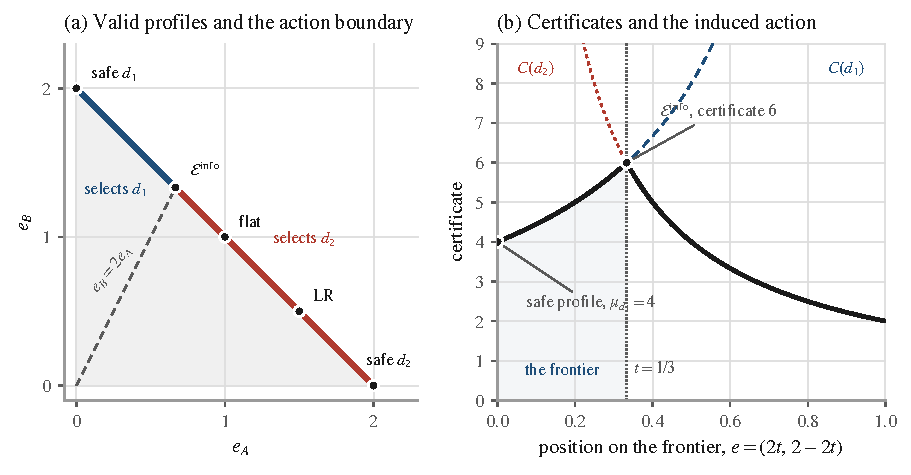
\includegraphics[width=0.92\textwidth]{toy_geometry.pdf}
\caption{Geometry of the two-outcome problem. Panel (a) shows the valid profiles and the action boundary, and panel (b) the two certificates along the budget line.}\label{fig:toy_geometry}
\end{figure}

Plotting the guarantee against the information gives the frontier in
Figure~\ref{fig:sim_frontier}. It is curved, so the exchange rate between the
two is not constant: the first units of certificate given up buy a great deal
of information, and the last buy very little. Most of the available
information can therefore be had for a modest loss of protection. The
protective endpoint itself is a limit of the curve rather than a point on it,
since the safe profile puts no e-value on $A$ and its log score is $-\infty$.

\begin{figure}[H]
\centering
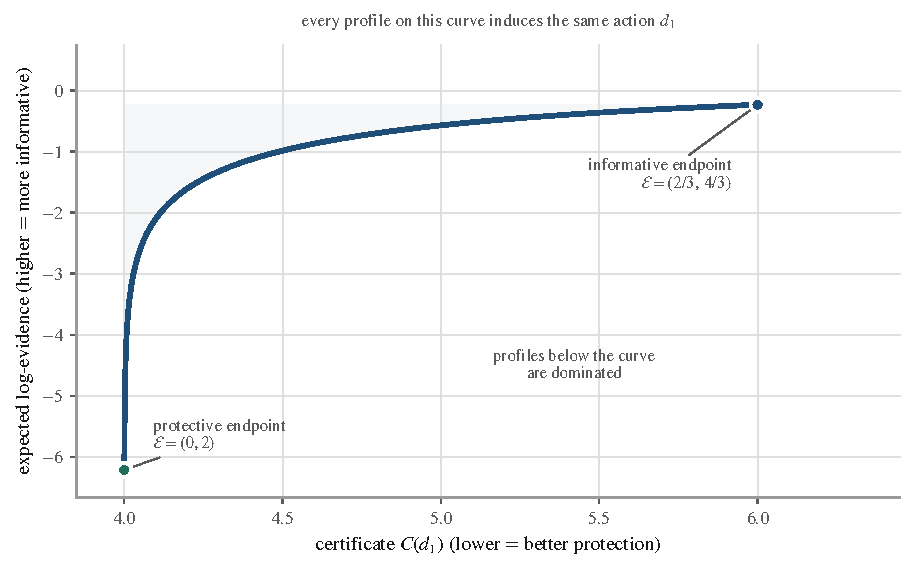
\includegraphics[width=0.92\textwidth]{sim_frontier.pdf}
\caption{The protection--information frontier for profiles inducing the bet on $A$.}\label{fig:sim_frontier}
\end{figure}

The same picture shows both cases of Proposition~\ref{prop:boundary}. Were
the target the hedge $d_2$, the likelihood ratio $(1.5,0.5)$, which sits at
$t=3/4$, would already lead to it, so the most informative profile for $d_2$
would be the ratio itself, with $d_2$ winning strictly at certificate $8/3$.
For the bet $d_1$ the ratio is out of reach, so the most informative profile
stops at the tie $t=1/3$. Which case applies depends only on whether the
likelihood ratio already leads to the target.

Where on the frontier to sit is a matter of preference, which the loss table
alone does not settle.

\subsection{Result 3: When Shape Functions Suffice}\label{sec:result3}

The first two results build profiles directly from the loss. The standard
construction never looks at the loss. It takes the likelihood ratio $r$ and
passes it through a shape function $w$, reporting $\mathcal E(z)=w(r(z))$.
Could a well-chosen shape function have produced the safe profile anyway? If
so, the loss would matter only for choosing $w$, and existing theory would
already cover the design problem.

There is a simple reason to doubt it. A shape function sees each outcome only
through its likelihood ratio, so two outcomes with the same ratio receive the
same score, however differently they cost. The safe profile scores outcomes
by their cost, so whenever two outcomes share a ratio but not a loss, no shape
function can reproduce it.

The shape functions used in practice come from the capped power family of
\citet{KoningvanMeer2025},
\begin{equation}
 w_h(r)=\min\!\left(\frac{r^{1/(1-h)}}{\lambda},\ \frac1\alpha\right).
 \label{eq:power_shape}
\end{equation}
It raises the ratio to a power, rescales it by the constant $\lambda$ that
makes the profile valid, and caps every score at $1/\alpha$. The parameter
$h<1$ sets how aggressively evidence is accumulated: $h=0$ returns the ratio
itself, and lower values flatten the profile. Different statisticians prefer
different $h$ and $\alpha$, but every member of the family reads each outcome
only through its ratio. The next result says exactly when that is enough.

\begin{proposition}[When shape functions suffice]\label{prop:no_shape}
Assume $\mu_d>0$, and let $r(z):=\widehat P_1(z)/P(z)$ be the likelihood ratio
against any fixed $P\in\mathcal P$ giving every outcome positive probability.
The safe profile $\mathcal E_d^{\mathrm{safe}}$ of
Theorem~\ref{thm:cert} can be written as $\mathcal E_d^{\mathrm{safe}}=w(r)$
for some function $w$ exactly when the loss is determined by the likelihood
ratio, meaning that
\[
  r(z)=r(z')\quad\text{implies}\quad L(d,z)=L(d,z')
\]
for every pair of outcomes $z,z'$.
\end{proposition}

\begin{proof}
Suppose first that $\mathcal E_d^{\mathrm{safe}}=w(r)$ for some $w$. If
$r(z)=r(z')$ then $w(r(z))=w(r(z'))$, so the two outcomes receive the same
e-value. Multiplying by $\mu_d$ recovers the loss, since
$L(d,\cdot)=\mu_d\,\mathcal E_d^{\mathrm{safe}}$, hence $L(d,z)=L(d,z')$.

Conversely, suppose the loss is constant on each level set of $r$. Define $w$
on the values $r$ actually takes by picking, for each such value $v$, any
outcome $z$ with $r(z)=v$ and setting
\[
  w(v)=\frac{L(d,z)}{\mu_d}.
\]
The choice of $z$ does not matter: any other outcome with the same ratio
carries the same loss by assumption, so $w$ is well defined. Off the range of
$r$ it may be given any values at all. By construction, at every outcome,
\[
  w(r(z))=\frac{L(d,z)}{\mu_d}=\mathcal E_d^{\mathrm{safe}}(z).
\]
\end{proof}

In words, a shape function can reproduce the safe profile exactly when
outcomes with the same likelihood ratio always carry the same loss. This can
fail in two different ways, and they should be kept apart.

The first is a failure of information. When two outcomes share a ratio but
differ in loss, nothing computed from the ratio can tell them apart, so no
shape function reproduces the safe profile, however it is chosen.

The second is subtler. When every outcome has its own ratio, the proposition
allows a suitable shape function to exist, but that function is only the loss
rewritten as a function of $r$ after the fact. A statistician choosing $w$
from preferences about evidence has no reason to arrive at it. Moreover, the
shape functions used in practice are increasing in $r$, so they give their
largest scores to the outcomes the belief rates likeliest relative to the
model, while the safe profile gives its largest scores to the outcomes where
the target is most expensive. When these are different outcomes, no
increasing shape can follow the safe profile, and
Section~\ref{sec:mkt_shape} shows a case where this alone puts the target out
of reach.

\subsection{The Procedure, Worked Through}\label{sec:recipe}

The three results combine into a procedure with three steps. First, compare
the actions and name the target. Second, build the safe profile for the
target. Third, if information matters, trade some protection for it while
keeping the target as a constraint. Each step is carried out below on the
two-outcome example, so every number can be checked by hand.

Step one compares the actions in the two ways a decision-maker might care
about, by worst-case expected loss across the model and by expected loss under
the belief. In the example,
\[
  \max_{P\in\mathcal P}\mathbb E_{P}[L(\cdot,Z)]
     =\bigl(\tfrac{0+8}{2},\tfrac{4+0}{2}\bigr)=(4,2),
  \qquad
  \mathbb E_{\widehat P_1}[L(\cdot,Z)]=(2,3),
\]
so the protective action is the hedge $d_2$, while the belief recommends the
bet $d_1$. The two differ, so the decision-maker has to choose. Take the bet
$d_1$ as the target, the choice of a belief-trusting decision-maker.
Everything that follows is conditional on that choice.

Step two builds the safe profile $L(d^\star,\cdot)/\mu_{d^\star}$. By
Theorem~\ref{thm:cert} it gives the target the strongest guarantee, and by
Corollary~\ref{cor:select} it leads to the target. For $d_1$, $\mu_{d_1}=4$
and $\mathcal E^{\mathrm{safe}}_{d_1}=(0,8)/4=(0,2)$, giving
\[
  C(d_1)=\max\bigl(0/0,\;8/2\bigr)=4,
  \qquad
  C(d_2)=\max\bigl(4/0,\;0/2\bigr)=\infty,
\]
under the conventions $0/0=0$ and $x/0=\infty$. The bet is selected. The
infinite certificate of the hedge is not an artefact. The safe profile puts
no e-value on $A$, the only outcome in which hedging costs anything, so that
loss is divided by zero rather than reduced.

Step three is optional. If the decision-maker also wants information, the
statistician moves along the frontier of Section~\ref{sec:frontier}, keeping
the target as a constraint. The most informative end is
$\mathcal E^{\mathrm{info}}=(2/3,4/3)$, with certificate $6$ instead of $4$ and
log score $-0.232$ instead of $-\infty$.

Table~\ref{tab:two_toy} collects the profiles. The two an evidence-first
statistician would report, the likelihood ratio and the flat profile, both
lead to the hedge. Only the profiles built from the loss of $d_1$ lead to the
bet. Each safe profile achieves its own action's best certificate and sends
the other action's to infinity, for the reason just seen.

\begin{table}[H]
\centering
\caption{Two-outcome profiles. $C_j$ is the certificate of action $d_j$.}\label{tab:two_toy}
\begin{tabular}{@{}l r r r r c@{}}\toprule
Profile & $\mathcal E(A)$ & $\mathcal E(B)$ & $C_1$ & $C_2$ & Action \\\midrule
Likelihood ratio & 1.50 & 0.50 & 16.00 & 2.67 & $d_2$ \\
Flat & 1.00 & 1.00 & 8.00 & 4.00 & $d_2$ \\
Safe for $d_2$ & 2.00 & 0.00 & $\infty$ & 2.00 & $d_2$ \\
Safe for $d_1$ & 0.00 & 2.00 & 4.00 & $\infty$ & $d_1$ \\
Informative for $d_1$ & 0.67 & 1.33 & 6.00 & 6.00 & $d_1$ \\\bottomrule
\end{tabular}
\end{table}

The last row is the informative profile. Its two certificates are equal, so
$d_1$ wins only through a tie, as Proposition~\ref{prop:boundary} predicts
when the likelihood ratio leads elsewhere. The three-outcome example behaves
the same way. Targeting $d_A$ there, the most informative profile is exactly
\[
  \mathcal E=\bigl(\tfrac95,\,\tfrac{12}{35},\,\tfrac67\bigr)
  \approx(1.80,\;0.34,\;0.86),
\]
with log score $+0.016$, and all three certificates equal
$35/3\approx11.67$, so $d_A$ ties with both competitors. A hand-picked profile that leans towards the draw,
$(0.3,0.7,2.0)$, also leads to $d_A$, and strictly, but scores $-0.760$.
Solving the constrained problem is therefore worth about $0.78$ in
log-evidence.

Every step of the procedure reads the loss. The likelihood ratio is still
worth reporting as a measure of evidence, but it is not a default the decision
should inherit.

%═══════════════════════════════════════════════════════════════════════════════
\section{Application: Stocking Shirts for the World Cup Final}\label{sec:market}
%═══════════════════════════════════════════════════════════════════════════════

Every example so far has stipulated its distributions. This section applies
the procedure of Section~\ref{sec:recipe} to real data, taking the belief from
Polymarket prices for the 2026 FIFA World Cup final between Spain and
Argentina \citep{Marketlens2026}. The decision-maker is a shopkeeper near the
stadium who orders replica shirts before the final and cannot reorder
afterwards. Shirts of the winning side sell and the rest are marked down. The
shopkeeper does not bet on the match and uses the prices only as a forecast,
so the cost of an order depends on how well it matches demand, never on the
prices themselves.

The section reaches one finding. Under the market's forecast the cheapest
order is mostly Spain shirts, yet no increasing reshaping of the likelihood
ratio leads to that order, across two extensive searches, while the safe
profile does. The reason is where each places its evidence. Protecting a
Spain-heavy order needs large scores on the Argentina outcomes, where that
order is ruinous. A reshaped likelihood ratio puts its largest score on a
Spain win within ninety minutes, where the market is most confident and the order
costs almost nothing. This is Result 2 in real data: the profile that best
reflects the belief leads away from the action the belief recommends.

\subsection{Two Contracts, Four Outcomes}\label{sec:mkt_data}

Two contracts were traded on the final, each settling on a different
question. A three-way result market pays out on the score after ninety
minutes, so a match still level then settles as a draw. A binary trophy
market pays out on whichever side eventually lifts the cup. Together they
tell the shopkeeper which side wins and whether the match is decided within
ninety minutes, and both affect how many shirts sell.

Figure~\ref{fig:market_odds} shows the two on one timeline. Prices are
recorded every minute of clock time, so breaks in play appear as gaps, which
is why the goal in the $106$th minute of play falls more than two hours after
kick-off. The two series part at the end of regulation. With the match level
the draw contract settles and the result market stops moving, while the
trophy market stays live and Spain's extra-time goal lifts their price from
about $0.60$ to over $0.90$. These are traded prices, not e-values.

\begin{figure}[H]
\centering
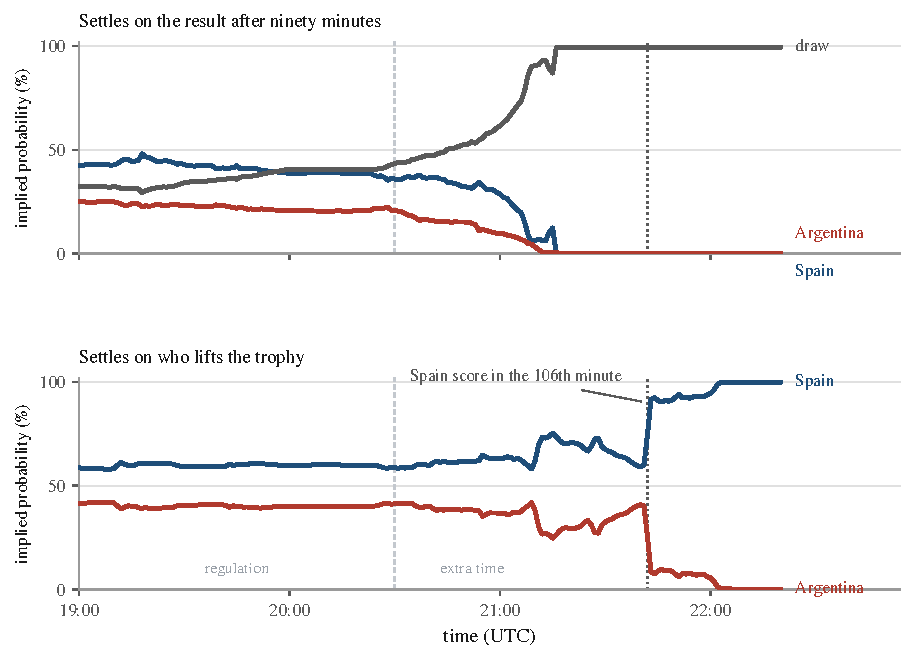
\includegraphics[width=0.92\textwidth]{polymarket_match_odds.pdf}
\caption{Two Polymarket contracts on the same match, from kick-off to settlement. The dashed line marks the end of regulation, the dotted line the goal.}\label{fig:market_odds}
\end{figure}

At kick-off the result market quoted
\[
  q=(0.4231,\;0.3238,\;0.2531)
\]
for a Spain win, a draw and an Argentina win, and the trophy market quoted
$o=(0.5863,\,0.4137)$ for Spain and Argentina. Each number is the midpoint of
the best bid and ask. Midpoints of separately traded contracts need not sum to
one, so each set is rescaled to sum to one, here and in
Figure~\ref{fig:market_odds}. The data also record how both contracts
settled: the draw contract paid out, and the trophy went to Spain
\citep{Marketlens2026}.

Read together, the two contracts describe four outcomes,
\[
  \mathcal Z=\{s,\;s^{\mathrm e},\;a,\;a^{\mathrm e}\},
\]
where $s$ is a Spain win within ninety minutes, $s^{\mathrm e}$ a Spain win
after extra time or penalties, and $a$ and $a^{\mathrm e}$ the same for
Argentina. Four outcomes need three numbers, and the two contracts supply
exactly three. The result market gives the two wins within ninety minutes
directly, and subtracting these from the trophy prices leaves the probability
of each side winning later:
\begin{equation}
  \widehat P_1(s)=q_1,\quad
  \widehat P_1(s^{\mathrm e})=o_1-q_1,\quad
  \widehat P_1(a)=q_3,\quad
  \widehat P_1(a^{\mathrm e})=o_2-q_3.
  \label{eq:market_ident}
\end{equation}
A match level after ninety minutes must eventually be won by someone, so the
two late wins should together account for the draw price, and they do:
$0.1632+0.1606=0.3238=q_2$. This holds by construction, since both sets of
prices were rescaled to sum to one, so it checks the arithmetic rather than
the market. The contracts cannot tell extra time from penalties, and nothing
below depends on that distinction.

These prices give the belief only. The model, the set of distributions the
guarantee must hold under, is not read from the prices at all. It is built
separately in the next subsection.

\subsection{The Model and the Belief}\label{sec:mkt_dists}

The procedure needs a belief and a model, and they do different jobs. The
belief is the shopkeeper's best guess at what will happen, and it decides
which order looks cheapest. The model is the set of distributions the
guarantee must hold up against, and it decides how strong a guarantee any
profile can give. Both must be fixed before kick-off, when the order is
placed.

The belief is the market's view at kick-off. Applying \eqref{eq:market_ident}
to the opening quotes gives
\[
  \widehat P_1=(0.4231,\;0.1632,\;0.2531,\;0.1606).
\]
Later prices cannot replace it. They absorb the match as it is played, and by
the end nearly all their probability sits on the outcome that happened, so
they report the result rather than forecast it.

The model needs more explanation. The guarantee is meant to hold even if the
market is wrong about this match, so the model cannot simply be the market's
forecast, or the guarantee would be only as good as the market. Instead it
collects a few distributions built from information available before the two
finalists were known, and the guarantee must hold under all of them.
These are not meant to be better forecasts than the market, which is better
informed. They are the alternatives the shopkeeper wants to be protected
against.

Each member splits the probability between the two sides, and then splits
each side between winning within ninety minutes and winning later. Three
splits between the sides are used: Polymarket's tournament-winner prices
early in the group stage, $0.138$ for Spain and $0.116$ for Argentina
\citep{PolymarketWinner2026}, rescaled to sum to one as
$(0.5433,0.4567)$, an even split, and $(0.45,0.55)$, leaning to Argentina. The share of matches decided later
comes from history. Of the twenty-one World Cup finals played as a single
deciding match between 1930 and 2022, eight went beyond ninety minutes
\citep{WCfinalsList}, a rate of $8/21=0.381$. The 1950 tournament is excluded
because it ended with a final group stage rather than a final. For the first
split this gives
\[
\begin{aligned}
  P&=\bigl(0.5433\,(0.619),\;0.5433\,(0.381),\;
             0.4567\,(0.619),\;0.4567\,(0.381)\bigr)\\
   &=(0.3363,\;0.2070,\;0.2827,\;0.1740),
\end{aligned}
\]
and the other two follow in the same way, so
\[
\begin{aligned}
  \mathcal P=\bigl\{&(0.3363,\;0.2070,\;0.2827,\;0.1740),\\
                    &(0.3095,\;0.1905,\;0.3095,\;0.1905),\\
                    &(0.2786,\;0.1714,\;0.3405,\;0.2095)\bigr\}.
\end{aligned}
\]

The model is deliberately more cautious than the belief. The market puts
$0.4231$ on a Spain win within ninety minutes, while no member of the model
goes above $0.3363$. By Theorem~\ref{thm:cert}, only one member matters for a
given order, the one under which that order looks worst, and
Section~\ref{sec:mkt_shape} checks that the findings survive changes to the
historical rate.

\subsection{The Two Criteria Disagree}\label{sec:mkt_decision}

The shopkeeper has room for one hundred shirts and must split them between the
two sides. Three orders are considered: mostly Spain ($d_1$, ninety Spain
shirts), an even split ($d_2$, fifty) and mostly Argentina ($d_3$, twenty).
Each shirt short of demand costs the lost margin, three units, and each shirt
left unsold costs the markdown, one unit.

Demand depends on the outcome. Only the winning side's shirts sell well, and a
win after extra time is a bigger occasion, so it sells more. Demand for the
winner's shirts is taken as eighty after a win within ninety minutes and one
hundred after a later win, with ten of the losing side either way. The cost of
each order then follows by arithmetic. In tens of units, for the outcomes
$(s,s^{\mathrm e},a,a^{\mathrm e})$,
\[
 L(d_1,\cdot)=(1,3,29,35),\quad
 L(d_2,\cdot)=(13,19,13,19),\quad
 L(d_3,\cdot)=(25,31,1,7).
\]

For example, ordering mostly Spain when Spain win within ninety minutes leaves
ten Spain shirts unsold, a cost of ten units, or $1$ in the table. Ordering
mostly Spain is cheap when Spain win and ruinous when Argentina do. The even
split is never cheap and never ruinous, and its cost depends only on when the
match is decided, not on who wins. No price appears anywhere in the table: the
market says what is likely, and the shirts say what it costs to be wrong.

Step one compares the orders in the two ways of Section~\ref{sec:recipe}, by
worst-case expected loss across the model and by expected loss under the
belief,
\[
\begin{aligned}
  \max_{P\in\mathcal P}\mathbb E_{P}[L(\cdot,Z)]&=(18.0000,\;15.2857,\;16.3251),\\
  \mathbb E_{\widehat P_1}[L(\cdot,Z)]&=(13.8738,\;14.9430,\;17.0142).
\end{aligned}
\]
The two disagree. The protective action is the even split $d_2$, the order
that cannot go badly wrong. The belief recommends mostly Spain, $d_1$, because
the market makes Spain the likelier winner. This is the case the thesis is
about.

Step two takes $d_1$ as the target, the choice of a belief-trusting
shopkeeper. The worst member of the model for $d_1$ is the one leaning to
Argentina,
\[
  P^\star=(0.2786,\;0.1714,\;0.3405,\;0.2095),
\]
under which
\[
  \mu_{d_1}=1\,(0.2786)+3\,(0.1714)+29\,(0.3405)+35\,(0.2095)=18.0000,
\]
so the safe profile of Theorem~\ref{thm:cert} divides the losses of $d_1$ by
$18$,
\begin{equation}
  \mathcal E^{\mathrm{safe}}_{d_1}
  =\frac{(1,3,29,35)}{18}
  =(0.0556,\;0.1667,\;1.6111,\;1.9444).
  \label{eq:market_safe}
\end{equation}
It puts most of its e-value on the two Argentina outcomes, where $d_1$ is most
exposed. Its certificate is $18$, and since $d_1$ is the action the belief
recommends, Corollary~\ref{cor:select} guarantees that it leads to $d_1$.
Table~\ref{tab:market} compares it with the profiles an evidence-first
statistician would report. The likelihood ratio there is taken against
$P^\star$ and scaled down by a factor of $1.051$, so that it is valid under
every member of the model.

\begin{table}[htbp]
\centering
\caption{The shopkeeper's order. Certificates $C_j$ of each order under each profile, the order the rule selects, and that order's expected loss under the kick-off belief.}\label{tab:market}
\begin{tabular}{@{}l r r r c r@{}}\toprule
Profile & $C_1$ & $C_2$ & $C_3$ & Action & $\mathbb E_{\widehat P_1}[L]$ \\\midrule
Likelihood ratio          & 48.002 & 26.058 & 34.233 & $d_2$ & 14.943 \\
Flat                      & 35.000 & 19.000 & 31.000 & $d_2$ & 14.943 \\
Safe for $d_2$            & 34.099 & 15.286 & 29.396 & $d_2$ & 14.943 \\
Safe for $d_1$            & 18.000 & 234.000 & 450.000 & $d_1$ & 13.874 \\\bottomrule
\end{tabular}
\end{table}

Only the safe profile for $d_1$ leads to $d_1$. The likelihood ratio and the
flat profile both leave the shopkeeper with the even split, and so does the
safe profile for $d_2$. This is the failure Section~\ref{sec:result2} warned
of: the likelihood ratio does not lead to the action the belief itself
recommends. Measured under the belief, that costs the shopkeeper about $1.07$
in expected loss, $14.943$ against $13.874$. The prediction-set rule of
Section~\ref{sec:intro_sets} does no better: at every coverage level from
$50\%$ to $95\%$ it also chooses the even split.

\subsection{No Increasing Shape Reaches the Target}\label{sec:mkt_shape}

Only the safe profile led to the order the belief recommends. A natural
objection is that the standard construction was not tried hard enough, and
that some other shape function would have led to $d_1$ as well. This
subsection shows that none does.

The standard construction reshapes the likelihood ratio of the belief against
the member of the model under which validity binds, here the worst member
$P^\star$, so
\[
  r=\frac{\widehat P_1}{P^\star}=(1.5188,\;0.9521,\;0.7433,\;0.7666).
\]
The ratio takes a different value at every outcome, so
Proposition~\ref{prop:no_shape} does not rule out writing the safe profile as
$w(r)$.

The obstacle is the second one described after that proposition. The
shape functions used in practice are increasing in $r$, so they rank the
outcomes as $r$ does,
\[
  a\ \prec\ a^{\mathrm e}\ \prec\ s^{\mathrm e}\ \prec\ s ,
\]
giving the most e-value to $s$, the outcome the belief rates likeliest
relative to the model. The loss of $d_1$ ranks them almost the other way,
\[
  s\ \prec\ s^{\mathrm e}\ \prec\ a\ \prec\ a^{\mathrm e} .
\]
To keep the certificate of $d_1$ low, the profile must put its largest
e-value on the two Argentina outcomes, where ordering mostly Spain is ruinous.
An increasing shape does the opposite. It puts its largest e-value on $s$,
where the order costs almost nothing, and its smallest on $a$ and
$a^{\mathrm e}$, where the order is most exposed. The safe profile
\eqref{eq:market_safe} reverses this, which is why it is not increasing in $r$.

Failing to match the safe profile exactly is not the same as failing to reach
$d_1$, so the question is settled by searching over shapes directly. Two
searches are run, both keeping every profile valid with its budget fully
spent, so that only the shape varies. The first covers the capped power
family \eqref{eq:power_shape} of Section~\ref{sec:result3}, sweeping $120$
values of $h$ in $[-6,0.95]$ against $60$ values of $\alpha$ in
$[0.01,0.95]$, a total of $7{,}200$ combinations, with $\lambda$ set by
bisection. The second drops the parametric form altogether. It draws
$200{,}000$ profiles by sampling four values uniformly, sorting them and
assigning them to the outcomes in increasing order of $r$, which gives a
random increasing shape.

Neither search ever reaches $d_1$. Every shape tried leads to the even split
or to mostly Argentina. Restricting to increasing shapes therefore does not
merely make $d_1$ more expensive to protect. It puts $d_1$ out of reach
altogether, while the safe profile reaches it with certificate $18$.

One input is left to the analyst, the historical rate at which finals go
beyond ninety minutes. Repeating the analysis for rates from $6/21$ to
$10/21$, two finals either side of the observed $8/21$, the two criteria
disagree at all five rates, and at all five no capped power shape reaches
$d_1$. The finding does not depend on that choice.

What the application cannot show is which criterion was right. Spain won
after extra time \citep{AlJazeera2026final}, the outcome $s^{\mathrm e}$, in which
ordering mostly Spain costs $3$ and the even split $19$. But a single match is
not a verdict on a decision rule. Settling that requires a setting where the
truth is known in advance.

%═══════════════════════════════════════════════════════════════════════════════
\section{Controlled Simulations: Scoring the Decisions Against a Known Truth}\label{sec:simulations}
%═══════════════════════════════════════════════════════════════════════════════

The application showed the two criteria disagreeing on real data, but a
single match cannot tell which of them was right. It produced one outcome,
and an order that was cheap this time could still be the worse choice on
average. Ranking decision rules needs the distribution
that generates the outcomes, which no real match supplies. This section
therefore runs controlled simulations, in which that distribution is fixed in
advance and every rule can be scored against it.

Each simulation adds a third distribution to the model and the belief, the
truth $P_{\mathrm{true}}$. It plays no part in choosing the action. Once an
action is chosen, it is scored by its expected loss under the truth,
\[
  \mathbb E_{P_{\mathrm{true}}}\bigl[L(\delta(\mathcal E),Z)\bigr].
\]
The truth need not lie in the model, since the model is what the
decision-maker wants protection against, not a claim about where the truth
lies.

The simulations compare four ways of choosing the evidence. Two follow the
procedure of Section~\ref{sec:recipe}, one targeting the action the belief
recommends and one targeting the protective action, and by
Corollary~\ref{cor:select} each takes its target. The other two are the
likelihood ratio and the flat profile, which take whatever action the rule
selects under them. The first simulation varies how confident the belief is,
the second how much worse a losing bet is than an unnecessary hedge, and the
third how wrong the belief is. Since every distribution is known, each
expected loss is exact.

\subsection{The Likelihood Ratio Moves Against the Belief}\label{sec:sim_belief}

The first simulation asks how each rule responds as the belief grows more
confident. Keep the two-outcome loss, with the bet $L(d_1,\cdot)=(0,8)$ and
the hedge $L(d_2,\cdot)=(4,0)$, hold the truth at $(0.75,0.25)$, and let the
belief put probability $p$ on $A$.

The belief's target is the bet when betting is cheaper under the belief,
$8(1-p)\leq4p$, that is $p\geq2/3$. More confidence in $A$ makes it readier to
bet, as one would expect. The likelihood ratio against $P_0=(1/2,1/2)$ is
$\mathcal E=(2p,2(1-p))$, with certificates
\[
  C(d_1;\mathcal E)=\frac{4}{1-p},
  \qquad
  C(d_2;\mathcal E)=\frac{2}{p},
\]
so it bets only when $p\leq1/3$. The two thresholds point in opposite
directions. The likelihood ratio bets on $A$ only when the belief makes $A$
unlikely, and above $p=2/3$, where betting is genuinely cheaper, it hedges,
more firmly the more confident the belief. Figure~\ref{fig:sim_belief} shows
the actions each rule takes and their expected loss under the truth.

\begin{figure}[H]
\centering
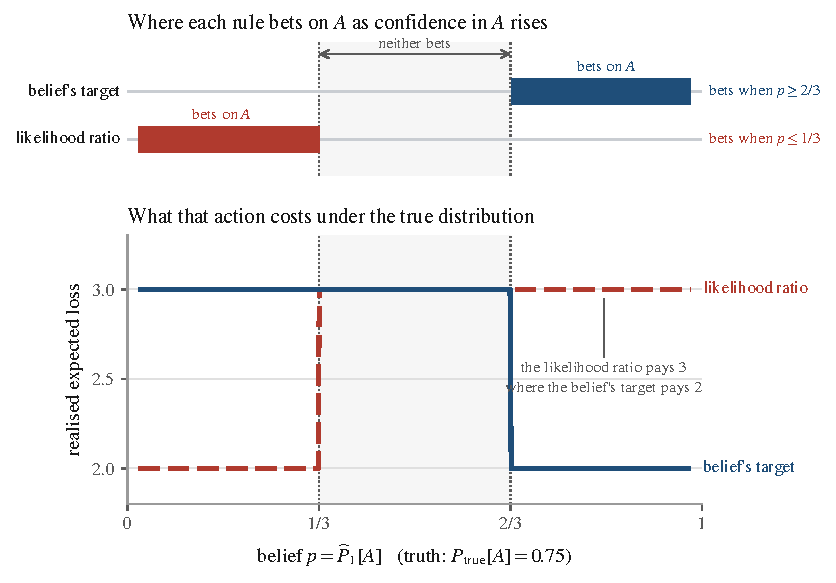
\includegraphics[width=0.92\textwidth]{sim_belief_sweep.pdf}
\caption{Actions taken and expected loss under the truth as confidence in $A$ varies. The procedure targeting the protective action and the flat profile hedge at every $p$, so only the two rules that ever bet are drawn.}\label{fig:sim_belief}
\end{figure}

This is the mechanism of Section~\ref{sec:result2} again. The likelihood
ratio puts large e-values on the outcomes the belief favours, so the rule
discounts the losses there. The bet loses only in $B$, which the belief
disfavours, so its loss is left undiscounted. That suits a profile meant as
evidence against the model, not one meant to act on a belief.

\subsection{How Wide the Disagreement Is}\label{sec:sim_window}

The second simulation varies the loss instead. Set the belief and the truth
both to $(0.75,0.25)$, so the belief is correct, and write $\ell$ for the
cost of a losing bet and $k$ for the cost of an unnecessary hedge, $8$ and $4$
in the example. With $p=0.75$, the bet is cheaper under the belief when
$\ell/k\leq p/(1-p)=3$, but the likelihood ratio selects it only when
$\ell/k\leq(1-p)/p=1/3$. In between, the likelihood ratio hedges although
betting is cheaper,
\begin{equation}
  \frac{1-p}{p}<\frac{\ell}{k}<\frac{p}{1-p},
  \qquad\text{here}\qquad \frac13<\frac{\ell}{k}<3.
  \label{eq:failure_window}
\end{equation}
The example's ratio of $2$ lies inside this window, which is why it separates
the two rules.

Since the belief is correct, the procedure targeting the belief's action has
the smallest expected loss at every ratio. What the simulation measures is the
width of the window, and \eqref{eq:failure_window} shows that it widens as the
belief grows more confident. Figure~\ref{fig:sim_window} plots the expected
losses and shades the window.

\begin{figure}[H]
\centering
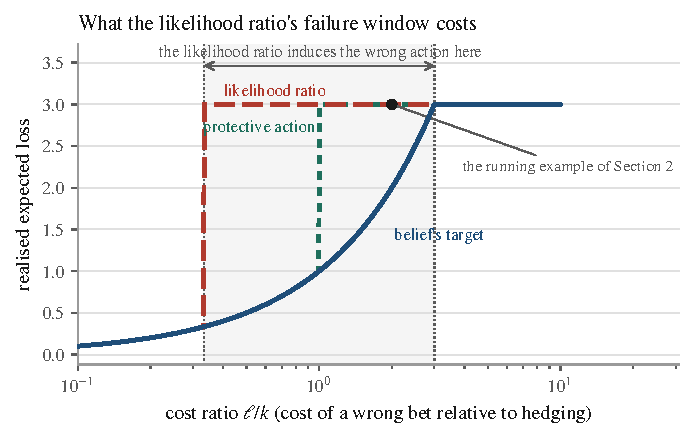
\includegraphics[width=0.92\textwidth]{sim_asymmetry_window.pdf}
\caption{Expected loss against the cost ratio $\ell/k$. Shading marks the window \eqref{eq:failure_window} in which the likelihood ratio takes the wrong action.}\label{fig:sim_window}
\end{figure}

\subsection{How Far an Optimistic Belief Can Be Trusted}\label{sec:sim_danger}

The first two simulations concern the profile: given a target, which action
does each profile lead to? This one concerns the target itself, which
Section~\ref{sec:choosing} leaves to the decision-maker's attitude toward risk.
It makes the belief wrong and asks how wrong it can be before trusting it
stops paying.

Take the three-outcome example of Section~\ref{sec:setup}, where the belief
$(0.6,0.3,0.1)$ puts only $0.1$ on the draw. Let the truth be
\[
  P_{\mathrm{true}}=\bigl(\tfrac23(1-c),\;\tfrac13(1-c),\;c\bigr),
\]
and raise the true probability $c$ of a draw from $0.01$ to $0.45$. The belief-trusting
procedure takes $d_A$ throughout, since the belief never changes, while the
guarantee-first procedure, the likelihood ratio and the flat profile all take
the insurance $d_C$. The expected losses of $d_A$ and $d_C$ under the truth
are equal at $c^*=1/4$. Below it trusting the belief costs less, and above it
insuring does.

The crossover comes well before the belief stops ranking the outcomes
correctly, since $A$ remains the most likely outcome until $c=2/5$. Ranking
correctly is not enough when the outcome the belief dismisses costs $10$. The
threshold comes from the loss table and the truth together. Draws are common
in football, so a belief that puts only $0.1$ on them may well be on the wrong
side of it.

The simulation does not say which target to name, since that depends on how
far the decision-maker trusts the belief. What it shows is what each choice
costs if the belief is wrong, which is exactly what a stated attitude toward
risk has to weigh.

Taken together, the simulations make a narrow point. The likelihood ratio can
take the wrong action even when the belief is exactly right, and over a wide
range of loss asymmetries. When the belief may be wrong, how far to trust it
depends on the loss table and the truth together, not on whether the belief
ranks the outcomes correctly.

What these simulations cannot do is show that the procedure decides better in
general, since their distributions are constructed rather than observed. That
is the price of knowing the truth at all, and Section~\ref{sec:disc_limits}
returns to it.

%═══════════════════════════════════════════════════════════════════════════════
\section{Conclusion}\label{sec:discussion}
%═══════════════════════════════════════════════════════════════════════════════

\subsection{What the Thesis Shows}\label{sec:disc_answer}

The loss must enter the construction of the evidence, not only its
interpretation. For a named target, the profile proportional to its loss is
the unique safest choice and leads to it. Information can be added only with
the target held as a constraint, since the likelihood ratio can lead
elsewhere even when the belief is right, and no reshaping of the ratio does
this job unless the loss is a function of it. The shopkeeper application
shows that this matters in practice.

When the model and the belief favour different actions, the disagreement
should be reported, since which to follow is the decision-maker's call.
Reporting the likelihood ratio alone, without the loss and the action it
induces, commits silently to an objective the decision may not share.

\subsection{Limitations}\label{sec:disc_limits}

Everything here is proved for finitely many outcomes. Theorem~\ref{thm:cert}
should extend to richer outcome spaces, but the thesis does not prove that,
and the frontier depends more on finiteness: with many actions or a continuum
of outcomes, both the existence of an optimum and the shape of the edges where
the target ties with a competitor need further assumptions.

Proposition~\ref{prop:boundary} also assumes that exactly one validity
constraint binds at the optimum. This holds for the one-point models it is
applied to, but with a composite model two constraints can bind at once, and
the most informative profile is then a compromise between members rather than
a ratio against any single one.

The information criterion is a choice, not a claim about what decision-makers
want. A different measure would move the interior of the frontier but not the
protective endpoint, so the target, and how much protection to trade for
information, must still be named by the decision-maker.

The empirical work is conditional too. The simulations construct their
distributions, so they show how the mechanism behaves rather than rank rules
in general. The application uses a real belief, but its loss table and model
are the analyst's choice. Section~\ref{sec:mkt_shape} varies the input that is
hardest to defend, the historical rate, and the finding survives, but a
different loss table could change it.

\subsection{Open Questions}\label{sec:disc_open}

Three questions remain open. The first is to extend the frontier beyond the
finite setting. The second is to find loss tables that are determined by the
likelihood ratio in practice, and to measure what is lost when they are not.
The third is how the model $\mathcal P$ should be chosen. It sets the strength
of every guarantee here, yet in the application it was assembled from
defensible judgements rather than derived from a principle.


% ── REFERENCES ───────────────────────────────────────────────────────────────
\newpage
\addcontentsline{toc}{section}{References}
\begingroup
% Long URLs need break freedom, but the entries themselves set justified and
% a little tighter, so the list does not spill an orphan onto its own page.
% Reference entries mix prose with unbreakable URLs, so a justified setting
% leaves loose lines at this measure. Ragged right keeps the word spacing even.
\sloppy
\setlength{\emergencystretch}{3em}
\raggedright
\setstretch{1.06}
\setlength{\bibsep}{0.7em}
% Reference list set one point below the 11pt body.
\fontsize{10}{12}\selectfont
\bibliography{bibliography}
\endgroup

% ── APPENDIX ─────────────────────────────────────────────────────────────────
\appendix
\newpage
%═══════════════════════════════════════════════════════════════════════════════
\section{Notation}\label{app:proofs}
%═══════════════════════════════════════════════════════════════════════════════

\begin{table}[htbp]
\centering
\caption{Notation used in the thesis.}
\small
\begin{tabular}{@{}l>{\raggedright\arraybackslash}p{0.72\textwidth}@{}}\toprule
Symbol & Meaning \\\midrule
$\mathcal Z$ & Outcome space \\
$\mathcal D$ & Action space \\
$\mathcal P$ & Model: the distributions validity must hold under \\
$P_0$ & The single member of a one-point model $\mathcal P=\{P_0\}$ \\
$\widehat P_1$ & Belief: the distribution the decision-maker thinks is true \\
$P_{\mathrm{true}}$ & Distribution generating outcomes in the simulations of Section~\ref{sec:simulations} \\
$P^\star$ & Member of $\mathcal P$ making the target action look worst \\
$L(d,z)$ & Loss of action $d$ when outcome $z$ occurs \\
$\mathcal E(z)$ & E-value assigned to candidate outcome $z$ \\
$r(z)$ & Likelihood ratio $\widehat P_1(z)/P^\star(z)$ \\
$w(\cdot)$ & Shape function, giving $\mathcal E(z)=w(r(z))$ \\
$w_h$ & Capped power shape with curvature $h$ and scale $\lambda$ \\
$S$ & Prediction set \\
$s,s^{\mathrm e},a,a^{\mathrm e}$ & Outcomes of the application: Spain or Argentina winning within ninety minutes, or later \\
$t$ & Share of the budget placed on $A$ along the two-outcome frontier \\
$C(d;\mathcal E)$ & Weighted worst-case certificate \\
$\mu_d$ & Worst expected loss $\max_{P\in\mathcal P}\mathbb E_{P}[L(d,Z)]$ \\
$\mathcal E_d^{\mathrm{safe}}$ & Safe profile for $d$, $L(d,\cdot)/\mu_d$ \\
$\mathcal E^{\mathrm{info}}$ & Constrained information-optimal profile \\
$\mathcal E^{\mathrm{flat}}$ & Flat profile, equal e-value at every outcome \\
$d^\star$ & Target action the profile is designed to induce \\
$\delta(\mathcal E)$ & Action selected by the weighted worst-case rule \\
$\alpha$ & Level at which a profile is thresholded, $\mathcal E\geq1/\alpha$, and the cap in $w_h$ \\
$\ell,k$ & Cost of a losing bet and of hedging, in Section~\ref{sec:sim_window} \\
\bottomrule\end{tabular}
\end{table}


\end{document}
